\section{Preliminary studies}

This section carries out some preliminary studies using Moltres and MOOSE heat conduction module to solve the prismatic HTGR thermal-fluids.

\subsection{Verification of the thermal-fluids model}

To verify our methodology, this section solved a simplified cylindrical model whose analytical solution we know.
The model assumes a sinusoidal power profile in the $z$-direction.
Section \ref{appendix:ver} presents the analytical solution of the problem.
Moltres/MOOSE obtained the numerical solution of equations in Section \ref{ch3:th}.

Figure \ref{fig:th-ver-mesh} displays the model geometry.
The model differentiates 5 subregions: fuel compact, helium gap, moderator, film, and coolant.
Table \ref{tab:th-ver-char} summarizes the geometry dimensions and the input parameters.
Data for a VHTR based on the GT-MHR.
The moderator thickness is the VHTR unit cell minimum distance between fuel and coolant channels.
We calculated the coolant radius by preserving the coolant channel volume.

\begin{table}[htbp!]
\centering
      \caption{characteristics.}
      \label{tab:th-ver-char}
    \begin{tabular}{@{}l c S[table-format=2.2] c c}
    \toprule
    \multicolumn{1}{c}{Parameter} & multicolumn{1}{c}{Symbol} & \multicolumn{1}{c@{}}{Value} & \multicolumn{1}{c@{}}{Units} & multicolumn{1}{c}{Reference} \\
    \midrule
  Fuel compact radius   & R$_f$     & 0.6225  & cm       & \cite{in_three-dimensional_2006} \\
  Fuel channel radius   & R$_g$     & 0.6350  & cm       & \cite{in_three-dimensional_2006} \\
  Coolant channel radius    & - 	& 0.7950  & cm       & \cite{in_three-dimensional_2006} \\
  Fuel/coolant pitch    & -			& 
  Fuel column height	& L 		& 793 	  & cm 		 & \cite{in_three-dimensional_2006} \\
  Coolant mass flow rate & $\dot{m}$ & 0.0176 & kg/s 	 & \cite{in_three-dimensional_2006} \\
  Average power density & q$_{ave}$ & 35      & W/cm$^3$ & \cite{in_three-dimensional_2006} \\
  Coolant inlet temperature 	& $T_{in}$ & 400  & $^{\circ}C$ & \cite{in_three-dimensional_2006} \\
  Helium inlet pressure & P 		& 70      & bar 	 & \cite{in_three-dimensional_2006} \\
  Helium density		& $\rho_c$  & 4.94 $\times 10^{-6}$ & kg/cm$^3$ & \cite{nist_thermophysical_2020} \\
  Helium heat capacity  & c$_{p,c}$	& 5.188 $\times 10^{3}$ & J/kg/K  & \cite{nist_thermophysical_2020} \\
  Fuel compact thermal conductivity & k$_f$ & 0.07    & W/cm/K & \cite{tak_numerical_2008} \\
  Gap thermal conductivity & k$_g$ & 3 \times 10^{-3} & W/cm/K & \cite{tak_numerical_2008} \\
  Moderator thermal conductivity & k$_m$ & 0.30 & W/cm/K 	& \cite{tak_numerical_2008} \\
    \midrule
  \multicolumn{1}{c}{Calculated parameters} &  &  &  & \\  
    \midrule
  Calculated moderator radius 	& R$_m$ & 1.08  		& cm     & - \\
  Coolant film radius   		& R$_i$ & 1.09  		& cm     & - \\
  Calculated coolant radius 	& R$_c$ & 1.349  		& cm     & - \\
  Coolant average velocity  	& v     & 1794.33 		& cm/s   & - \\
  Film thermal conductivity  	& k$_i$ & 1.722 $\times 10^{-3}$ & W/cm/K & - \\
  \bottomrule
  \end{tabular}
\end{table}

Figure \ref{fig:th-ver-results} shows the axial and radial temperature profiles.
Both analytical and numerical solutions exhibit good agreement.
The outlet coolant temperature is 770.2 $^{\circ}$C whereas the average outlet coolant temperature of the VHTR is 950 $^{\circ}$C.
Note that this is a simplified model only for verification purposes, and it considers only one fuel channel while in the GT-MHR unit cell two fuel channels deposit their heat in one coolant channel.

\begin{figure}[htbp!]
	\centering
	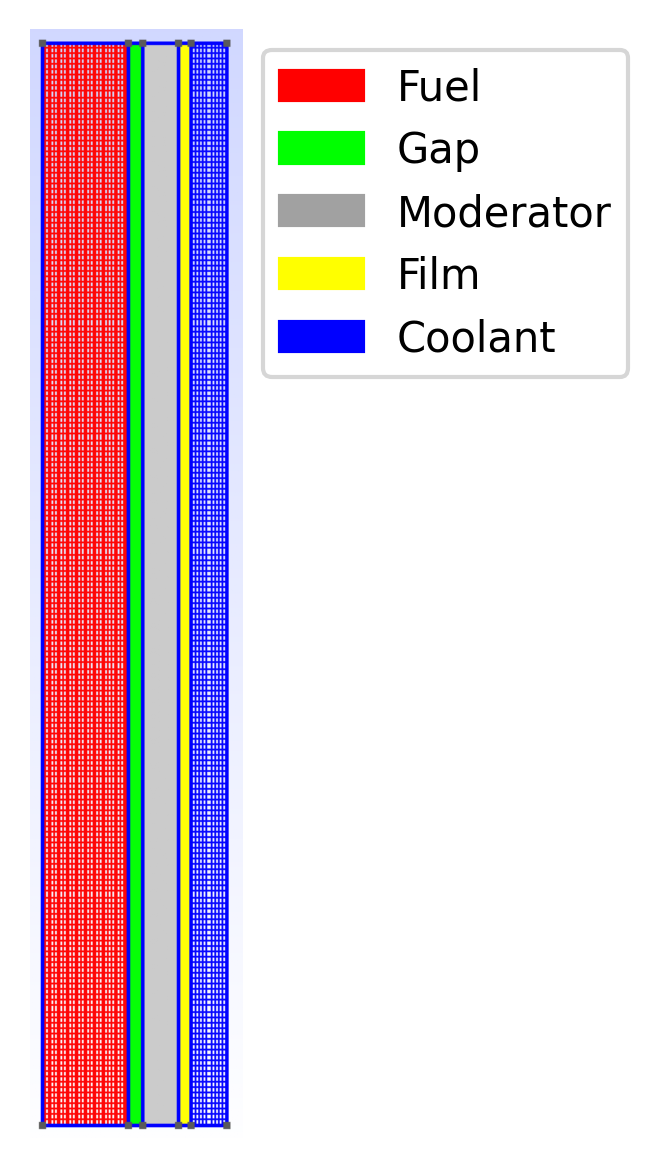
\includegraphics[width=0.3\linewidth]{figures-thermal/2D-preliminar-mesh2}
	\hfill
	\caption{Scaled-down version of the model geometry.}
	\label{fig:th-ver-mesh}
\end{figure}

\begin{figure}[htbp!]
	\centering
    \subfloat[Fuel centerline and bulk coolant axial temperatures. \label{fig:th-ver-results-a}]{
        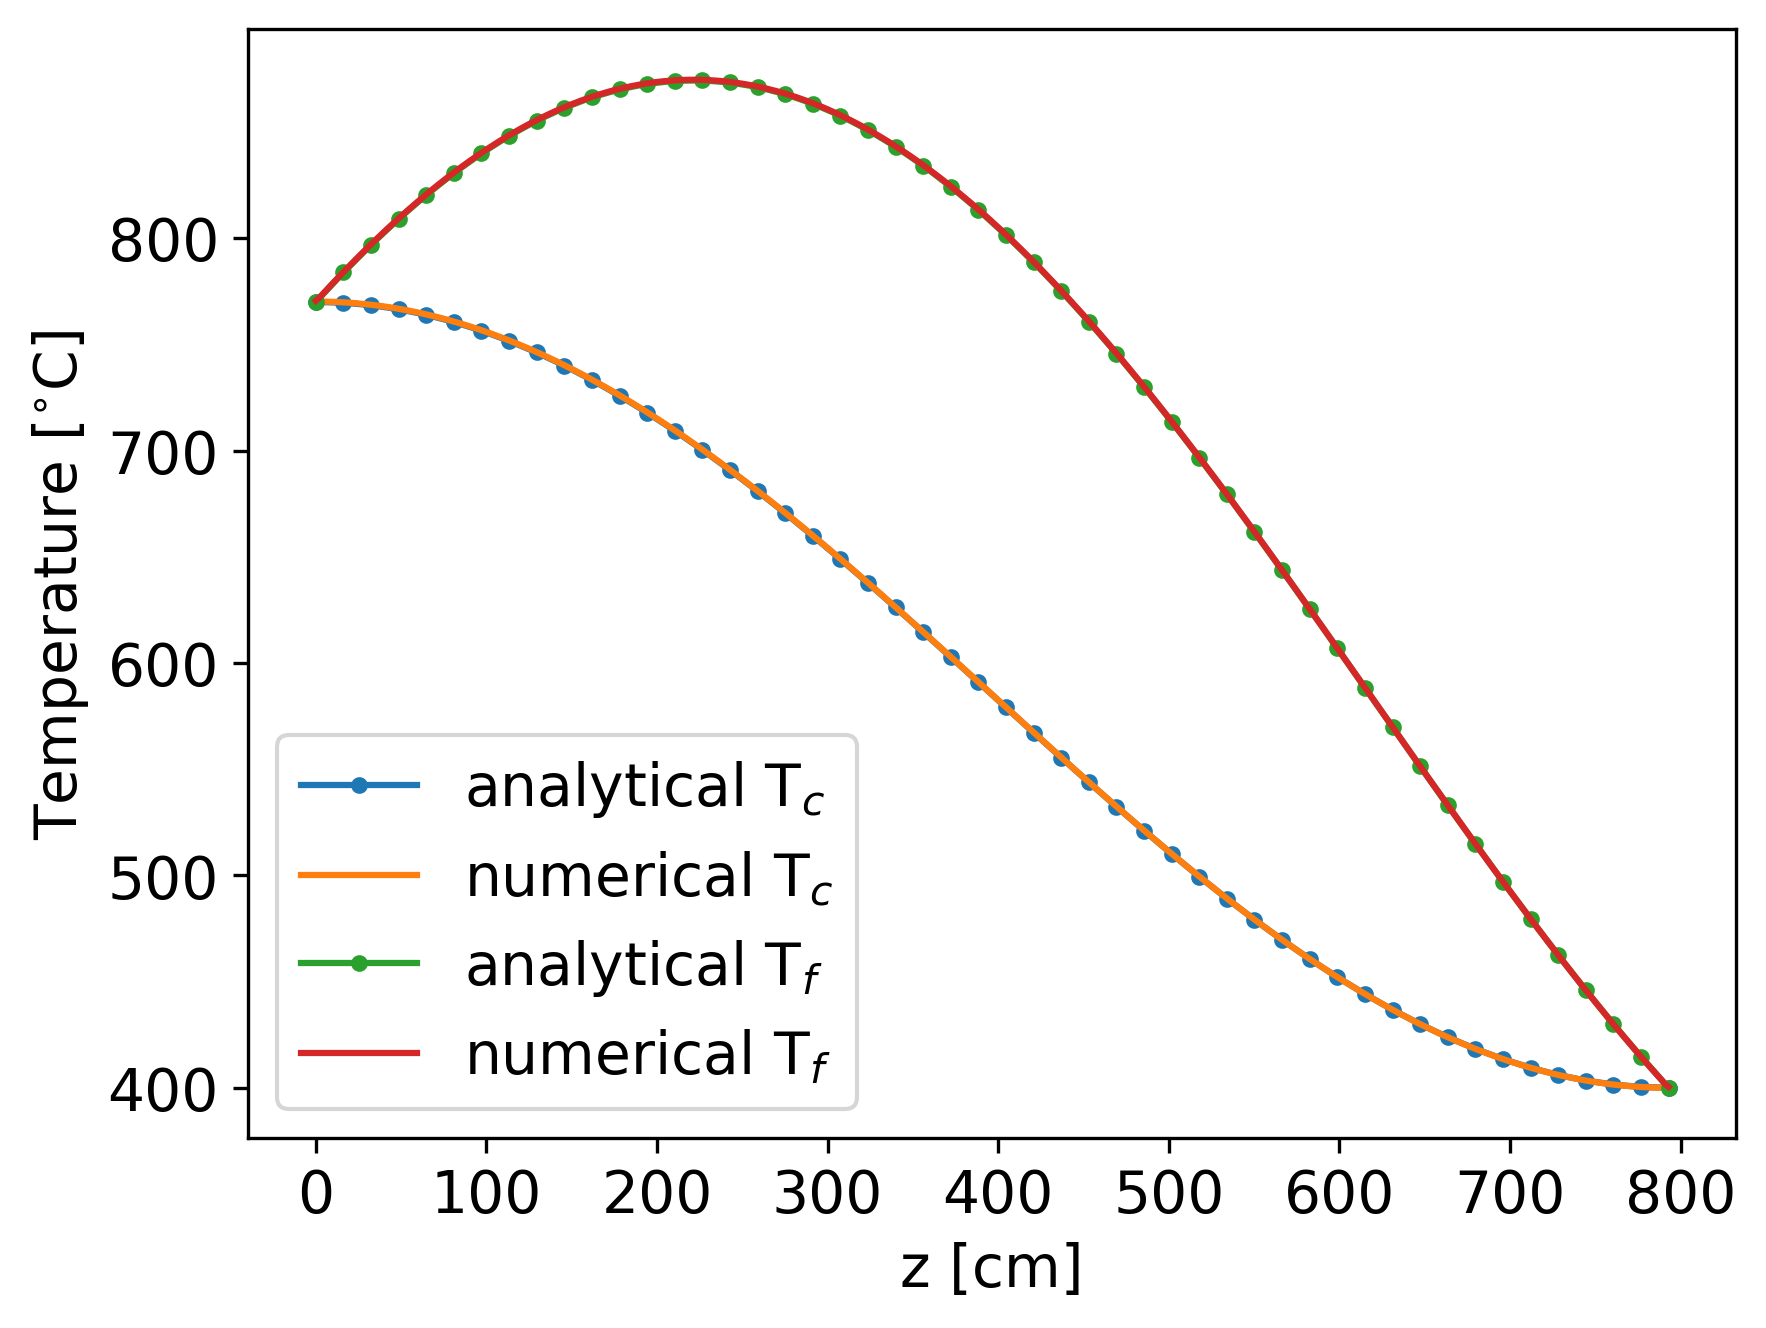
\includegraphics[width=0.45\textwidth]{figures-thermal/2D-preliminar-axial}
    }
    \subfloat[Radial temperature at z=396.5 cm.]{
        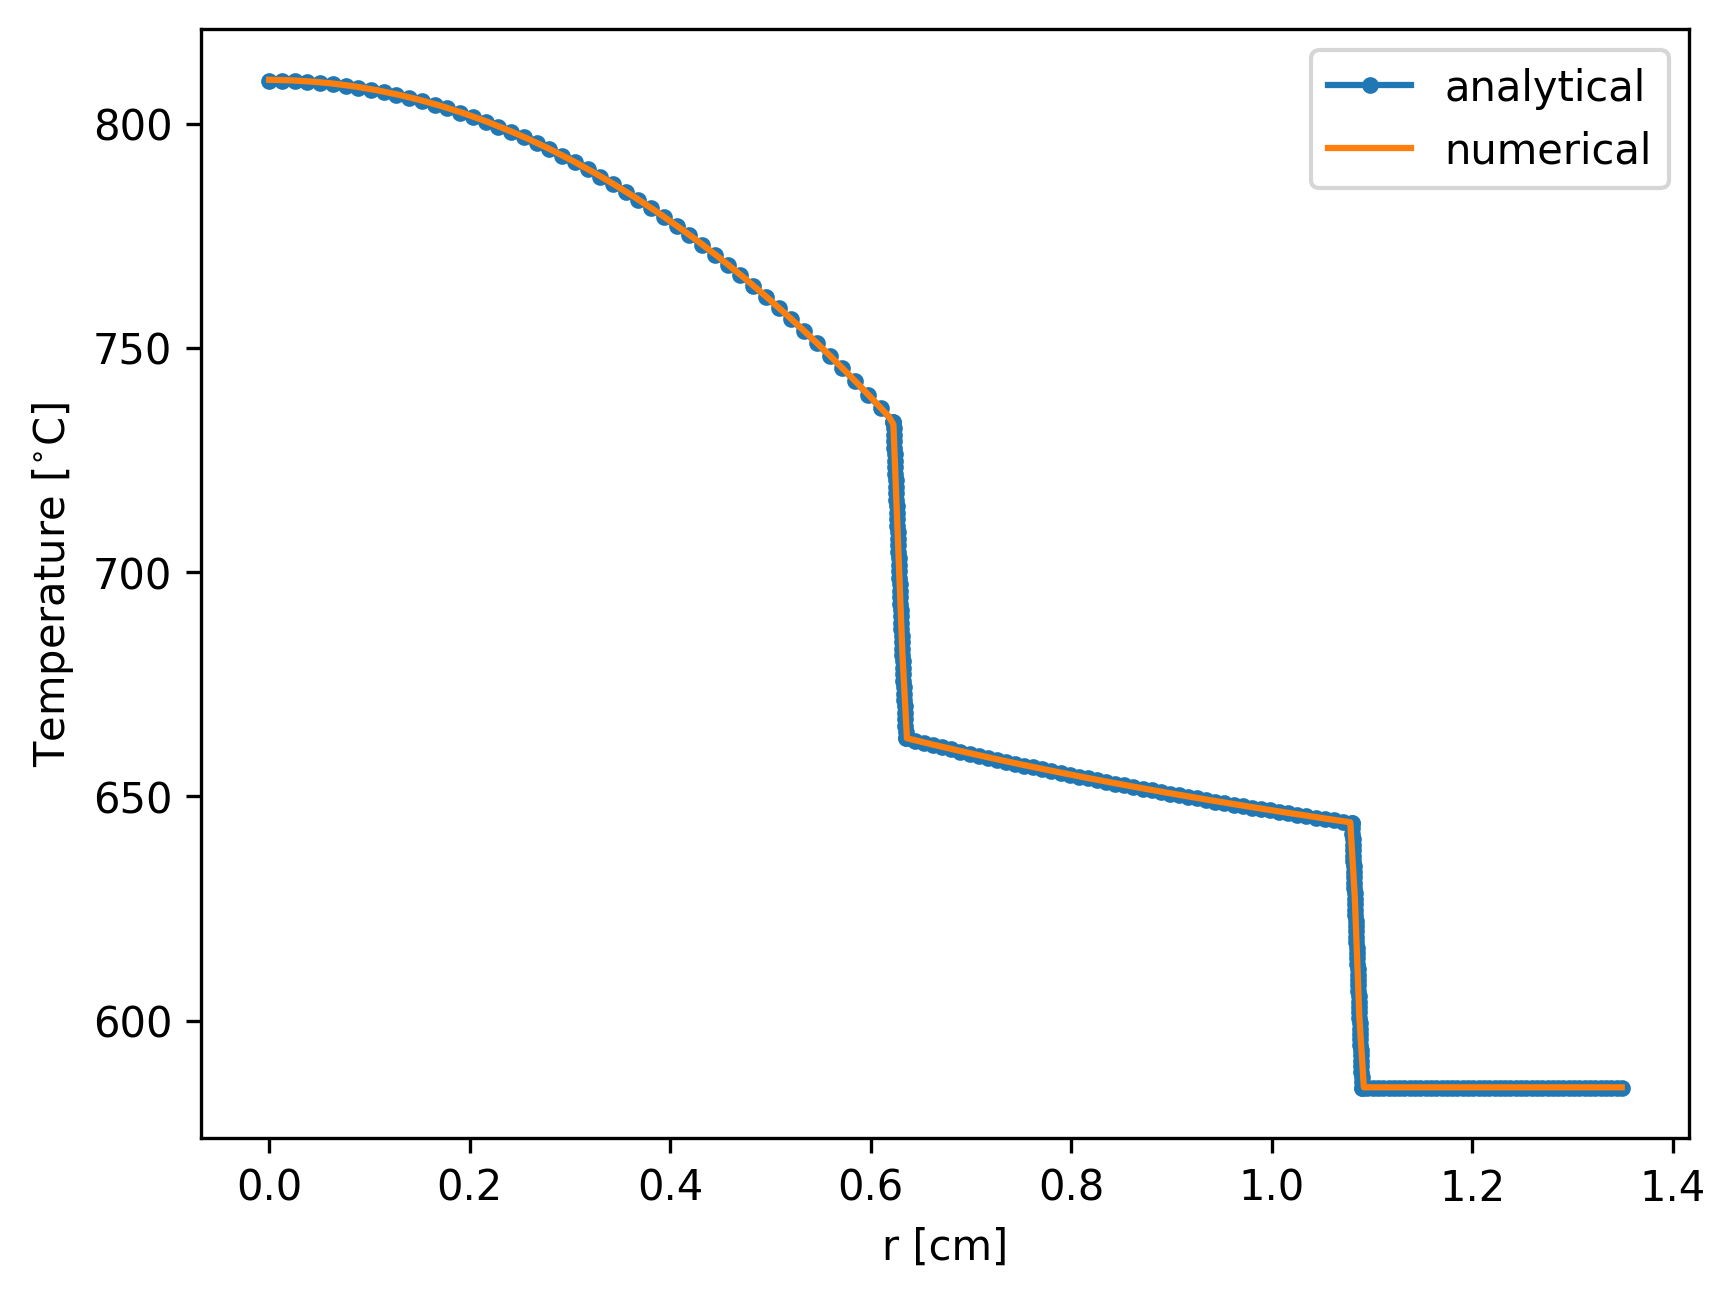
\includegraphics[width=0.45\textwidth]{figures-thermal/2D-preliminar-radial}
    }
	\hfill
    \caption{Temperature profiles.}
	\label{fig:th-ver-results}
\end{figure}

\section{Unit cell problem}

This section will solve the unit cell problem in the hot spot of an HTGR.
Intends to reproduce \cite{in_three-dimensional_2006}.
Missing material properties come from \cite{tak_numerical_2008}.
The material properties vary with the temperature (both in In et al and my simulation).

\begin{table}[htbp!]
\centering
      \caption{characteristics.}
      \label{tab:th-ver-char}
    \begin{tabular}{@{}l c S[table-format=2.2] c c}
    \toprule
    \multicolumn{1}{c}{Parameter} & multicolumn{1}{c}{Symbol} & \multicolumn{1}{c@{}}{Value} & \multicolumn{1}{c@{}}{Units} & multicolumn{1}{c}{Reference} \\
    \midrule
  Fuel compact radius       & R$_f$ & 0.6225    & cm   & \cite{in_three-dimensional_2006} \\
  Fuel channel radius       & R$_g$ & 0.6350    & cm   & \cite{in_three-dimensional_2006} \\
  Coolant channel radius    & R$_c$ & 0.7950    & cm   & \cite{in_three-dimensional_2006} \\
  Fuel/coolant pitch        & p     & 1.885     & cm   & \cite{in_three-dimensional_2006} \\
  Fuel column height        & L     & 793       & cm   & \cite{in_three-dimensional_2006} \\
  % input parameter characteristics
  Coolant channel mass flow rate & $\dot{m}$ & 0.0176 & kg/s & \cite{in_three-dimensional_2006} \\
  Average power density     & q$_{ave}$ & 35    & W/cm$^3$   & \cite{in_three-dimensional_2006} \\
  Inlet coolant temperature & T$_{in}$  & 400   & $^{\circ}$C  & \cite{in_three-dimensional_2006} \\
  Helium inlet pressure & P & 70 & bar & \cite{in_three-dimensional_2006} \\
  Helium density        & \rho  & 4.94 $\times 10^{-6}$ & kg/cm$^3$ & \cite{nist_thermophysical_2020} \\
  Helium heat capacity  & c$_p$ & 5188 & J/kg/K & \cite{nist_thermophysical_2020} \\
    \midrule
  \multicolumn{1}{c}{Calculated parameters} &  &  &  & \\  
    \midrule
  Coolant film radius       & R$_i$ & 0.8050    & cm   & -\\
  Film thermal conductivity & k_$i$ & 0.001731 & W/cm/K & - \\
  \bottomrule
  \end{tabular}
\end{table}

\begin{figure}[htbp!]
	\centering
    \subfloat[Model geometry.]{
        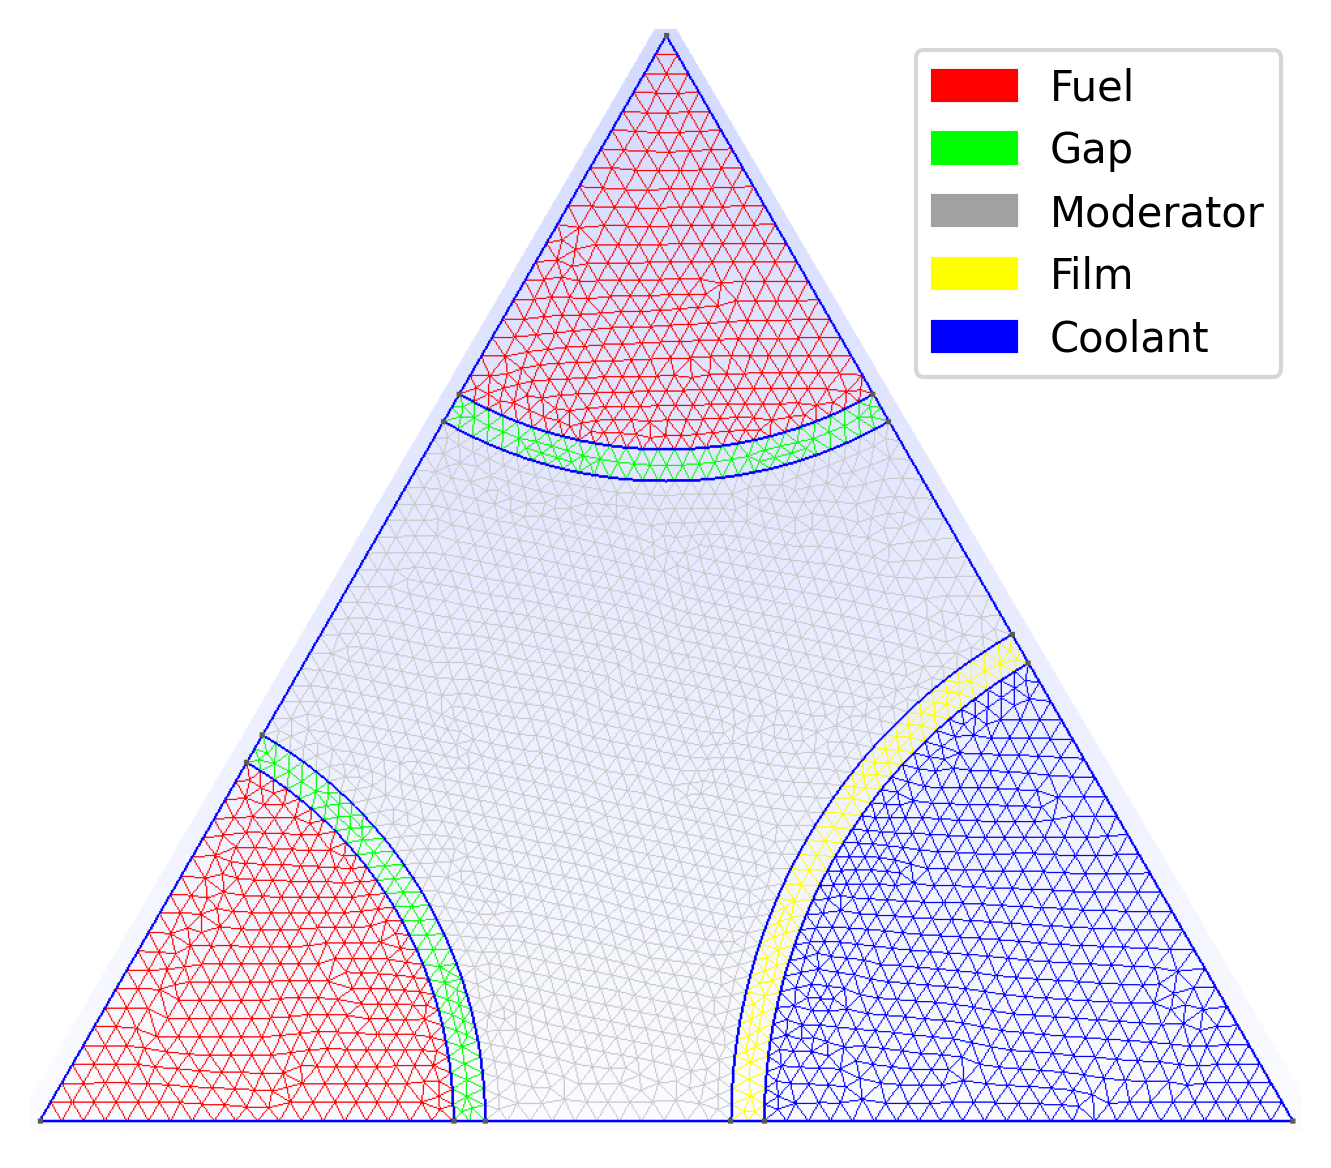
\includegraphics[width=0.45\textwidth]{figures-thermal/3D-unitcell-mesh}
    }
    \subfloat[Material properties.]{
        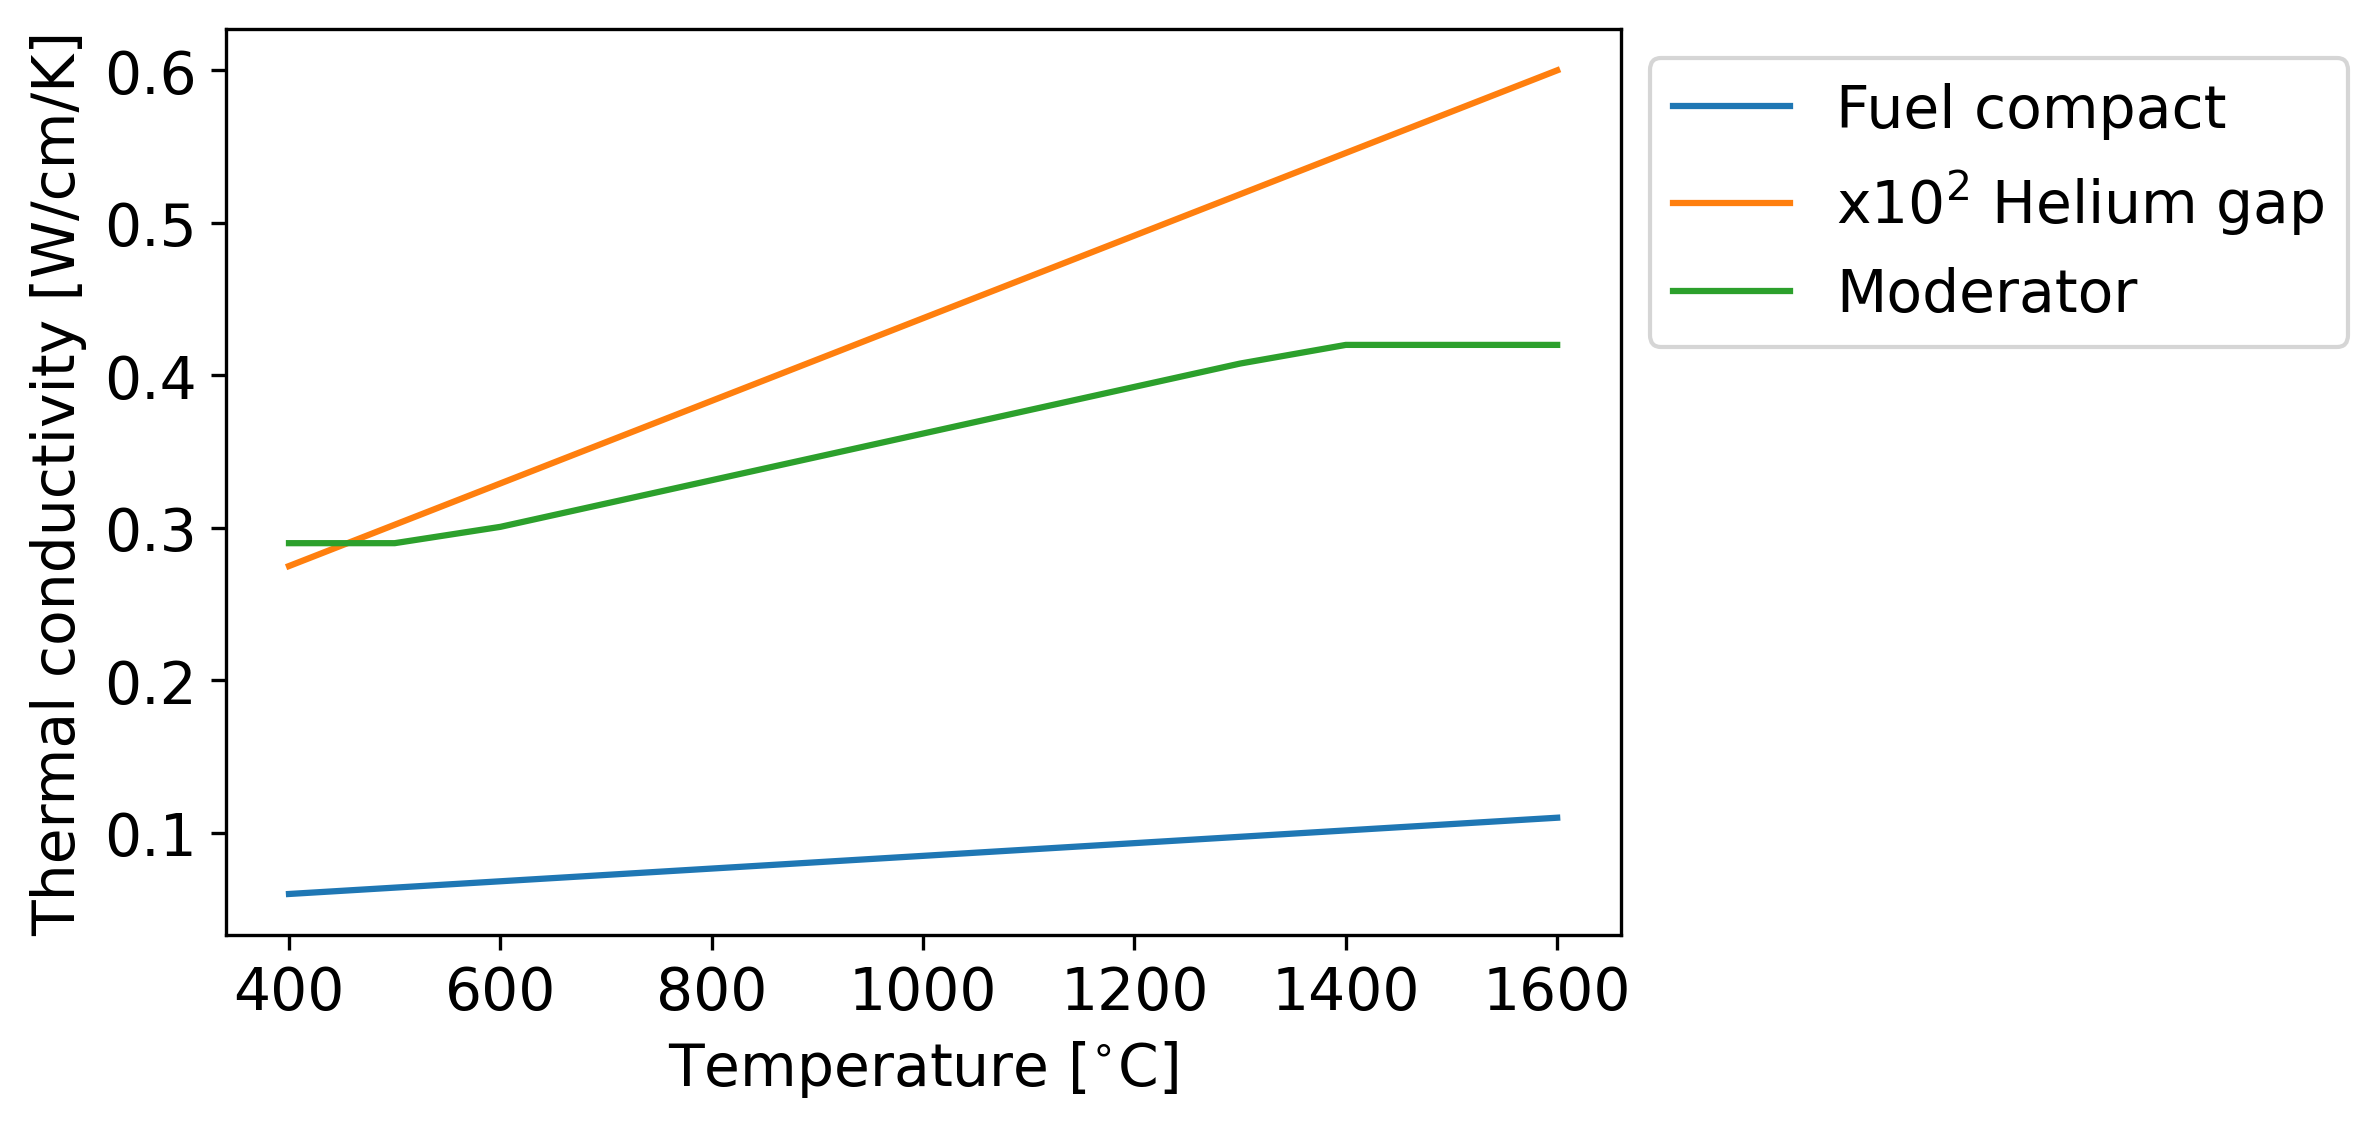
\includegraphics[width=0.45\textwidth]{figures-thermal/val-unit-matprop}
    }
	\hfill
    \caption{.}
	\label{fig:th-val-uni-results}
\end{figure}

\section{Fuel assembly}

This section will calculate the heat profile of a fuel assembly of a HTGR.

\section{Full core}

This section will extend the methodology to a full-ore problem and it will intend to solve Exercise 2 of Phase I of the OECD/NEA MHTGR-350 Benchmark.




\section{Neutronics and Thermal-fluids Coupling}

3 options:
- Heterogeneous model
- Homogenized media and sub-channel unit cell model: how does it solve advection ?
- Porous media model


